\documentclass[12pt,a4paper]{article}

% ── Packages ───────────────────────────────────────────────────────────────
\usepackage[margin=2.5cm, headheight=15pt]{geometry}
\usepackage{graphicx}
\usepackage{comment}
\usepackage{hyperref}
\usepackage{listings}
\usepackage{xcolor}
\usepackage{tikz}
\usetikzlibrary{shapes.geometric, arrows.meta, positioning, fit, backgrounds, decorations.pathreplacing}
\usepackage{booktabs}
\usepackage{caption}
\usepackage{parskip}
\usepackage{titlesec}
\usepackage{fancyhdr}
\usepackage{amsmath}

% ── Page style ─────────────────────────────────────────────────────────────
\pagestyle{fancy}
\fancyhf{}
\rhead{Assignment 1 -- Q1}
\lhead{OSI Model Encapsulation}
\cfoot{\thepage}

% ── Listing style (C code) ─────────────────────────────────────────────────
\definecolor{codebg}{RGB}{245,245,245}
\definecolor{keywordcolor}{RGB}{0,0,200}
\definecolor{commentcolor}{RGB}{60,130,60}
\definecolor{stringcolor}{RGB}{180,0,0}

\lstdefinestyle{cstyle}{
    language=C,
    backgroundcolor=\color{codebg},
    basicstyle=\ttfamily\small,
    keywordstyle=\color{keywordcolor}\bfseries,
    commentstyle=\color{commentcolor}\itshape,
    stringstyle=\color{stringcolor},
    numberstyle=\tiny\color{gray},
    numbers=left,
    stepnumber=1,
    numbersep=8pt,
    frame=single,
    framerule=0.4pt,
    breaklines=true,
    breakatwhitespace=false,
    tabsize=4,
    showstringspaces=false,
    captionpos=b,
}

% ── TikZ styles ────────────────────────────────────────────────────────────
\tikzset{
    layer/.style={
        rectangle, rounded corners=4pt,
        minimum width=8.5cm, minimum height=0.9cm,
        text centered, draw=black, thick,
        font=\sffamily\small
    },
    app/.style    ={layer, fill=blue!20},
    pres/.style   ={layer, fill=cyan!20},
    sess/.style   ={layer, fill=teal!20},
    tran/.style   ={layer, fill=green!25},
    net/.style    ={layer, fill=yellow!30},
    dl/.style     ={layer, fill=orange!30},
    phy/.style    ={layer, fill=red!20},
    arrow/.style  ={-{Stealth[length=6pt]}, thick},
    hdrlabel/.style={font=\ttfamily\tiny, text=gray, right=0.15cm}
}

\title{ECE F343: Communication Networks \\ \large{Assignment 1 - Question 1}}
\author{Pranav Chandra N. V. \\ 2023AAPS0013P}
\date{26/06/2026}
% ── Document ───────────────────────────────────────────────────────────────
\begin{document}
\maketitle
\tableofcontents
\newpage

\section{Introduction}

This program was written for Assignment 1, Question 1. The goal is to show
how message encapsulation works in the OSI model by simulating the
downward flow of data from Layer 7 (Application) to Layer 1 (Physical).

The user enters a message of up to 80 characters. The program passes it
through seven functions, one per layer. Each function sticks its own header
onto the front of whatever it received, prints the result, and then calls
the function for the layer below it.

\section{OSI Reference Model Overview}

The OSI model splits network communication into seven layers, each with a
specific job. Table~\ref{tab:osi} lists each layer, the name for its unit
of data (PDU), and the header string used in this program.

\begin{table}[h!]
	\centering
	\caption{OSI Layers, PDU names, and simulated headers}
	\label{tab:osi}
	\begin{tabular}{clll}
		\toprule
		\textbf{Layer} & \textbf{Name} & \textbf{PDU} & \textbf{Simulated Header}                             \\
		\midrule
		7              & Application   & Message      & \texttt{[APP: HTTP GET /index.html]}                  \\
		6              & Presentation  & Message      & \texttt{[PRES: ENC=UTF-8 FORMAT=ASCII COMPRESS=NONE]} \\
		5              & Session       & Message      & \texttt{[SESS: ID=A1B2C3 SEQ=001 TYPE=DATA]}          \\
		4              & Transport     & Segment      & \texttt{[TRAN: TCP SRC=1234 DST=80 SEQ=100 ACK=0]}    \\
		3              & Network       & Packet       & \texttt{[NET: SRC=192.168.1.1 DST=10.0.0.1 TTL=64]}   \\
		2              & Data Link     & Frame        & \texttt{[DL: SRC=AA:BB:CC DST=11:22:33 TYPE=IPv4]}    \\
		1              & Physical      & Bits         & \texttt{[PHY: ENC=NRZ SIGNAL=DIGITAL]}                \\
		\bottomrule
	\end{tabular}
\end{table}

% ═══════════════════════════════════════════════════════════════════════════
\section{Program Design}
% ═══════════════════════════════════════════════════════════════════════════

\subsection{Design Decisions}

\begin{itemize}
	\item A helper function \texttt{prepend\_header()} takes care of copying
	      the header and message into a new buffer, so the layer functions
	      themselves stay short and readable.
	\item Buffers are fixed-size arrays on the stack (\texttt{MAX\_BUF = 1024}
	      bytes). This is more than enough for seven headers plus an 80-char
	      message, and the helper exits if that ever overflows.
	\item All headers are kept under 64 characters as required by the spec.
	\item Each layer function just calls the one below it directly, keeping
	      the call chain simple and easy to follow.
\end{itemize}

\newpage
\subsection{Constants and Macros}

\begin{lstlisting}[style=cstyle, caption={Buffer and header constants}]
#define MAX_APP_MSG  80    
#define MAX_HEADER   64   
#define MAX_BUF      1024

#define HDR_APP   "[APP: HTTP GET /index.html]"
#define HDR_PRES  "[PRES: ENC=UTF-8 FORMAT=ASCII COMPRESS=NONE]"
#define HDR_SESS  "[SESS: ID=A1B2C3 SEQ=001 TYPE=DATA]"
#define HDR_TRAN  "[TRAN: TCP SRC=1234 DST=80 SEQ=100 ACK=0]"
#define HDR_NET   "[NET: SRC=192.168.1.1 DST=10.0.0.1 TTL=64]"
#define HDR_DL    "[DL: SRC=AA:BB:CC DST=11:22:33 TYPE=IPv4]"
#define HDR_PHY   "[PHY: ENC=NRZ SIGNAL=DIGITAL]"
\end{lstlisting}

\subsection{Helper: \texttt{prepend\_header()}}

\begin{lstlisting}[style=cstyle, caption={Header prepending helper}]
static int prepend_header(const char *header, const char *msg, int msg_size, char *out_buf, int out_buf_size){
    int hdr_len  = (int)strlen(header);
    int new_size = hdr_len + msg_size;

    if (new_size >= out_buf_size) {
        fprintf(stderr, "Buffer overflow prevented.\n");
        exit(1);
    }

    memcpy(out_buf,           header, hdr_len);
    memcpy(out_buf + hdr_len, msg,    msg_size);
    out_buf[new_size] = '\0';

    return new_size;
}
\end{lstlisting}

\subsection{Layer Functions}

All seven layer functions work the same way:

\begin{enumerate}
	\item Allocate a local buffer (\texttt{MAX\_BUF} bytes).
	\item Call \texttt{prepend\_header()} to build the new PDU.
	\item Print it.
	\item Call the next layer down (the Physical layer skips this last step).
\end{enumerate}

\newpage
\begin{lstlisting}[style=cstyle, caption={Application Layer (representative example)}]
void application_layer(char *msg, int size)
{
    char buf[MAX_BUF];
    int  new_size = prepend_header(HDR_APP, msg, size, buf, MAX_BUF);
    printf("[Layer 7 - Application]  PDU: %s\n\n", buf);
    presentation_layer(buf, new_size);
}
\end{lstlisting}

% ═══════════════════════════════════════════════════════════════════════════
\section{Message Flow Flowchart}
% ═══════════════════════════════════════════════════════════════════════════

Figure~\ref{fig:flowchart} shows the message moving down through the layers.
The PDU gets longer at each step as another header is added to the front.

\begin{figure}[h!]
	\centering
	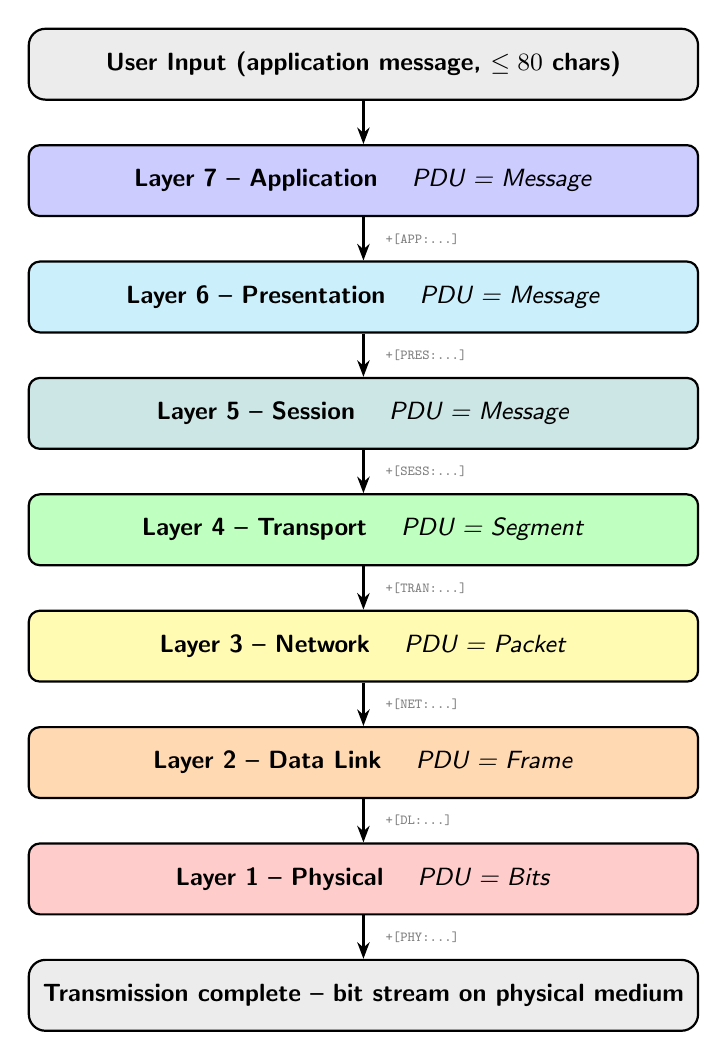
\begin{tikzpicture}[node distance=0.55cm and 2cm]

		% ── Input ──────────────────────────────────────────────────────────────
		\node[rectangle, rounded corners=6pt, draw, fill=gray!15, thick,
			minimum width=8.5cm, minimum height=0.9cm,
			font=\sffamily\small\bfseries] (input)
		{User Input (application message, $\leq 80$ chars)};

		% ── Layers ─────────────────────────────────────────────────────────────
		\node[app,  below=of input]  (L7) {\textbf{Layer 7 -- Application}  \quad\textit{PDU = Message}};
		\node[pres, below=of L7]     (L6) {\textbf{Layer 6 -- Presentation} \quad\textit{PDU = Message}};
		\node[sess, below=of L6]     (L5) {\textbf{Layer 5 -- Session}      \quad\textit{PDU = Message}};
		\node[tran, below=of L5]     (L4) {\textbf{Layer 4 -- Transport}    \quad\textit{PDU = Segment}};
		\node[net,  below=of L4]     (L3) {\textbf{Layer 3 -- Network}      \quad\textit{PDU = Packet}};
		\node[dl,   below=of L3]     (L2) {\textbf{Layer 2 -- Data Link}    \quad\textit{PDU = Frame}};
		\node[phy,  below=of L2]     (L1) {\textbf{Layer 1 -- Physical}     \quad\textit{PDU = Bits}};

		% ── Output ─────────────────────────────────────────────────────────────
		\node[rectangle, rounded corners=6pt, draw, fill=gray!15, thick,
			minimum width=8.5cm, minimum height=0.9cm,
			font=\sffamily\small\bfseries, below=of L1] (output)
		{Transmission complete -- bit stream on physical medium};

		% ── Arrows ─────────────────────────────────────────────────────────────
		\draw[arrow] (input) -- (L7);
		\draw[arrow] (L7)    -- node[hdrlabel] {\texttt{+[APP:...]}} (L6);
		\draw[arrow] (L6)    -- node[hdrlabel] {\texttt{+[PRES:...]}} (L5);
		\draw[arrow] (L5)    -- node[hdrlabel] {\texttt{+[SESS:...]}} (L4);
		\draw[arrow] (L4)    -- node[hdrlabel] {\texttt{+[TRAN:...]}} (L3);
		\draw[arrow] (L3)    -- node[hdrlabel] {\texttt{+[NET:...]}} (L2);
		\draw[arrow] (L2)    -- node[hdrlabel] {\texttt{+[DL:...]}} (L1);
		\draw[arrow] (L1)    -- node[hdrlabel] {\texttt{+[PHY:...]}} (output);
		\begin{comment}

		% ── Encapsulation brace label ───────────────────────────────────────────
		\draw [decorate, decoration={brace, amplitude=6pt}, thick, gray]
		([xshift=4.5cm] L7.north east) -- ([xshift=4.5cm] L1.south east)
		node [midway, right=10pt, font=\sffamily\scriptsize, text=gray,
			align=center] {Each layer\\prepends\\its header};

		\end{comment}

	\end{tikzpicture}
	\caption{Message flow and encapsulation across the OSI 7 layers.}
	\label{fig:flowchart}
\end{figure}

% ═══════════════════════════════════════════════════════════════════════════
\newpage
\section{Sample Output}

Running the program with the input \texttt{"Hello, Network!"} gives:

\begin{lstlisting}[style=cstyle, language={}, caption={Sample program output}]
Enter application message (up to 80 characters):
> Hello, Network!

=== OSI Encapsulation ===

[Layer 7 - Application]  PDU: [APP: HTTP GET /index.html]Hello, Network!

[Layer 6 - Presentation] PDU: [PRES: ENC=UTF-8 FORMAT=ASCII COMPRESS=NONE][APP: HTTP GET /index.html]Hello, Network!

[Layer 5 - Session]      PDU: [SESS: ID=A1B2C3 SEQ=001 TYPE=DATA][PRES: ...]...[APP: ...]Hello, Network!

[Layer 4 - Transport]    Segment: [TRAN: TCP SRC=1234 DST=80 SEQ=100 ACK=0][SESS: ...]...[APP: ...]Hello, Network!

[Layer 3 - Network]      Packet: [NET: SRC=192.168.1.1 DST=10.0.0.1 TTL=64][TRAN: ...]...Hello, Network!

[Layer 2 - Data Link]    Frame: [DL: SRC=AA:BB:CC DST=11:22:33 TYPE=IPv4][NET: ...]...Hello, Network!

[Layer 1 - Physical]     Bits: [PHY: ENC=NRZ SIGNAL=DIGITAL][DL: ...]...Hello, Network!

=== Transmission complete: 271 bytes on the wire ===
\end{lstlisting}

% ═══════════════════════════════════════════════════════════════════════════
\section{Build and Run}
% ═══════════════════════════════════════════════════════════════════════════

The project uses a simple \texttt{Makefile}:

\begin{lstlisting}[style=cstyle, language=make, caption={Makefile}]
CC     = gcc
CFLAGS = -Wall -Wextra -std=c11
TARGET = osi_model
SRC    = osi_model.c

all: $(TARGET)

$(TARGET): $(SRC)
    $(CC) $(CFLAGS) -o $(TARGET) $(SRC)

clean:
    rm -f $(TARGET)
\end{lstlisting}

Compile and run with:
\begin{lstlisting}[style=cstyle, language=bash]
make
./osi_model
\end{lstlisting}

% ═══════════════════════════════════════════════════════════════════════════
\section{Conclusion}
% ═══════════════════════════════════════════════════════════════════════════

This program gives a rough idea of how encapsulation works going down the
OSI stack. Each layer adds its own header before passing the data on, so
by the time it reaches Layer 1 the original message is buried inside
several headers. The headers here are simplified --- they do not carry real
protocol data --- but the structure matches what each layer is actually
responsible for: application requests at Layer 7, encoding info at Layer 6,
session tracking at Layer 5, port and sequence numbers at Layer 4, IP
addresses at Layer 3, MAC addresses at Layer 2, and signalling info at
Layer 1.

\end{document}
